\documentclass{article}
\usepackage[utf8]{inputenc}
\usepackage[margin=1in]{geometry}
\usepackage{courier}
\usepackage{graphicx}
\graphicspath{ {images/} }

\setlength{\parskip}{\baselineskip}%
\setlength{\parindent}{0pt}%
\title{ECE559 Table Final Report}
\author{Jiawei Zhang, Alan Guo, Phil Foo, Diane Kim }
\date{December 16, 2016}

\begin{document}

\maketitle

\section{Summary}

The table subsystem can be thought of as a map from 48-bit MAC addresses to port information that can store up to 32 entries. The table interfaces directly with the forwarding subsystem and provides a mechanism to store port information related to specific previously-stored MAC addresses.

\section{High-level Description}

Functions of the table subsystem include processing frame data to determine which port, if any, each frame information should the forwarding subsystem forward to. The table subsystem’s functions are executed during either write state, or read state. Under write state, the table first looks up the source address provided by forwarding. If the given source address already exists in the table, it updates the port information and its priority tag. If the given source address does not exist in the table, it gets added to the table. If the table is already full, an entry with the lowest priority tag will get evicted.

The only subsystem of the switch that the table interfaces with is forwarding. In fact, the table is located inside the forwarding subsystem, which means that it receives inputs from forwarding, and also outputs its results to forwarding. Forwarding provides source address and source port pairs to store and also inputs destination addresses. Then the table returns corresponding destination port ID or asserts \texttt{monitor\_not\_found} signal. Our subsystem also provides two signals to monitoring subsystem: \texttt{monitor\_not\_found} and \texttt{monitor\_access}.

IEEE Standards 802.3 on Ethernet states various specifications on 1 Gigabit Ethernet switch. Although most specifications apply to the external interfaces only, our table subsystem still abides by specifications stated in the IEEE standards. Table provides simple management interfaces by using simple 1 bit signals to communicate with forwarding such as \texttt{trigger}, \texttt{input\_ready}, \texttt{output\_ready} . Also, table uses 1 hot encoding to simplify port ID information. One other relevant constraints that IEEE standard notes is that forwarding operation must complete within 82 cycles in order to support 100Mb/s rates for data transfer and management functions. Table function only takes 3 cycles to operate in order to support this specification.  

\newpage

\section{Design Description}

The table subsystem is designed with modularity and ease-of-use in mind. The implementation takes advantage of VHDL language features including subtyping and keep memory and logic gate constraints in mind. 

\subsection{Inter-subsystem Interface}

The table subsystem receives all of its input signals from the forwarding subsystem and outputs signals to forwarding and monitoring (through forwarding). Table~\ref{tab:a} shows the signal names of the inter-subsystem interface. The interface is defined in \texttt{address\_table.vhd}.

\begin{table}[ht]
    \begin{center}
        \begin{tabular}{lrll}\hline
        Signal & Width & In/Out & Used By \\
        \hline
        \texttt{clock} & 1 & In & Forwarding \\
        \hline
        \texttt{reset} & 1 & In & Forwarding \\
        \hline
        \texttt{source\_address} & 48 & In & Forwarding \\
        \hline
        \texttt{source}\_port & 4 & In & Forwarding \\
        \hline
        \texttt{destination\_address} & 48 & In & Forwarding \\
        \hline
        \texttt{trigger} & 1 & In & Forwarding \\
        \hline
        \texttt{destination\_port} & 4 & Out & Forwarding \\
        \hline
        \texttt{output\_ready} & 1 & Out & Forwarding \\
        \hline
        \texttt{input\_ready} & 1 & Out & Forwarding \\
        \hline
        \texttt{monitor\_access} & 1 & Out & Monitoring \\
        \hline
        \texttt{monitor\_not\_found} & 1 & Out & Monitoring \\
        \hline
        \end{tabular}
        \caption{Table Inter-Subsystem Interface}\label{tab:a}
    \end{center}
\end{table}

\subsubsection{Signal Description}

The \texttt{clock} signal comes from the forwarding subsystem and is used to clock the FSMs and memory elements within the table subsystems. The positive \texttt{clock} edge also serves as a control signal to latch \texttt{source\_address}, \texttt{source\_port}, and \texttt{destination\_address} values when \texttt{trigger} is asserted. The maximum time required to perform a lookup and store operation is two clock cycles counted from the positive \texttt{clock} edge when the input trigger is asserted. The table subsystem is designed to work with the 50 MHz clock passed from forwarding, but any PLL divided clock signal will still work. 

The \texttt{reset} signal is an active-high asynchronous clear that resets the all the stored destination address to 0 and all the stored one-hot destination port values to 0, which is designed to be an invalid value. 

The \texttt{source\_address} signal is a 48-bit logic vector that represents a source MAC address. The signal is the key to be stored in the table and maps to a port. It is latched on the positive \texttt{clock} edge when \texttt{trigger} is asserted.

The \texttt{source\_port} signal is a 4-bit logic vector that represents the source port. The logic vector is one-hot encoded. The vector can be used in the direction as forwarding wishes, with either port 1 mapping to the MSB or port 1 mapping to the LSB. The value is latched on the positive \texttt{clock} edge when \texttt{trigger} is asserted.

The \texttt{destination\_address} signal is a 48-bit logic vector that represents a destination MAC address. The signal is the key used to look up a port in the table. It is latched on the positive \texttt{clock} edge when \texttt{trigger} is asserted.

When the single-bit \texttt{trigger} signal is asserted and a positive \texttt{clock} edge occurs, the \texttt{source\_address}, \texttt{source\_port}, and \texttt{destination\_address} are latched. 

The \texttt{destination\_port} signal is a 4-bit logic vector that represents the looked-up destination port. If the destination address is found, the destination port is returned in the same format as the source port was originally specified in. If the destination address is not found, the destination port takes on the hardcoded value "1111", which tells the forwarding subsystem to forward to all four ports. The \texttt{destination\_port} signal is only valid on the positive edge of the \texttt{output\_ready} signal.

The \texttt{output\_ready} signal's positive edge denotes when the \texttt{destination\_port} signal contains a valid value or a not-found value ("1111"). The \texttt{output\_ready} signal is guaranteed to be asserted within two cycles of the \texttt{trigger} signal being asserted at a positive \texttt{clock} edge. 

The \texttt{output\_ready} signal is asserted when the table is ready for a new load-store operation. This signal is guaranteed to be asserted within three cycles of the \texttt{trigger} signal being asserted at a positive \texttt{clock} edge. This signal can be disregarded if the \texttt{trigger} signals are asserted on positive \texttt{clock} edges at least three cycles apart. 

The \texttt{monitor\_access} signal is used to show that a load-store operation has been performed. 

The \texttt{monitor\_not\_found} signal is used to show that a destination address was not found in the table. This always occurs at least once during the operation of the table during the initial load-store operation since the value we are trying to load will not exist (unless we consider the MAC address 00-00-00-00-00-00 which will in practice not appear). For both \texttt{monitor\_access} and \texttt{monitor\_not\_found} signals, the signal is guaranteed to be asserted for no longer than a single clock cycle at a time and the signal should be considered only at the positive clock edge. For every load-store operation, the signals are guaranteed to be asserted at only one positive clock edge from the positive clock edge when the \texttt{trigger} is asserted to when the \texttt{input\_ready} signal is asserted.

\newpage
\subsection{Subsystem Design}

The overall design of the table subsystem is completely original and no external sources were consulted besides VHDL language constructs. On a high level, a chain of 32 52-bit register files is used to store 52-bit vectors composed of 48-bit MAC address vectors and 4-bit port vectors. The register chain is essentially a shift register that shifts from the left-most (31st register file) to right-most (1st register file). For each load-store operation, the load is performed first, followed by the store. The load parallel-queries the 32 52-bit register files and compares the destination address with the 48-bit MAC addresses stored in the register files. If the address is found, the associated 4-bit port is returned and all the register files to the left of it plus itself assert their write-enable and take the value of the register file to the left. The left-most register file takes the value of the register-file where the destination address was found. If the address is not found, the port "1111" is returned and the table is not changed. This simulates an LRU function for the load operation. 

The store operation behaves similarly. If the source address is found in the table, then the register file which the source address is found in has its source port updated. Then, like in the load operation, all register files to the left of it plus itself assert their write-enable and take the value of the register file to the left. The left-most register file then takes the value of the register-file with the updated port. When the source address is not found in the table, then all register files have their write-enable asserted and the new source address and port and placed in the left-most register file. This operation evicts the least recently used address and port. Note that eviction can only occur on stores as the load operation always feeds the shifted-out value back into the left-most register file.

\texttt{monitor\_access} is always asserted after the load operation commences. The \texttt{monitor\_not\_found} signal is asserted after the load operation is attempted and the address is not found.

\subsection{Intra-subsystem Interfaces}

In order to simplify implementation of the table subsystem, the subsystem was abstracted into several high-level modules. These modules each represent a fundamental portion of the table subsystem and they were partitioned with the simplicity of interfaces between them in mind. 

\newpage
\subsubsection{Block Diagram}
The block diagram of table is shown in Figure~\ref{fig:block_diagram} shows interfaces between four main modules and one internal wrapper process module which selects and outputs appropriate values to internal signals according to FSM states. For example, this process module selects source address as an address to compare during the write state instead of destination address. 
\begin{figure}[ht!]
  \centering
  	\includegraphics[width=0.95\textwidth]{block_diagram.png}
  \caption{Block diagram of the whole table subsystem}
  \label{fig:block_diagram}
\end{figure}


\subsubsection{Register Chain Module}

The register chain module consists of 32 52-bit register files, each of which stores a 48-bit MAC address and a 4-bit port. The module takes a 32-bit write-enable signal to control the write-enables for each of the 52-bit register files. the module also takes a 52-bit input for the left-most register. The only output is a 32 by 52 vector array of the contents of the register files in the register chain. The register chain module implementation is in \texttt{register\_chain.vhd}. Table~\ref{tab:reg} shows the signal names of the intra-subsystem interface. 


\begin{table}[ht]
    \begin{center}
        \begin{tabular}{lll}\hline
        Signal & Type & In/Out \\
        \hline
        \texttt{rc\_clock} & std\_logic & In \\
        \hline
        \texttt{rc\_reset} & std\_logic & In \\
        \hline
        \texttt{rc\_first\_value} & std\_logic\_vector(51 downto 0) & In \\
        \hline
        \texttt{rc\_write\_enable} & std\_logic\_vector(31 downto 0) & In \\
        \hline
        \texttt{rc\_reg\_output} & reg\_output\_type & Out \\
        \hline
        \end{tabular}
        \caption{Register Chain Interface}\label{tab:reg}
    \end{center}
\end{table}

The \texttt{rc\_clock} and \texttt{rc\_reset} signals are the same signals as the inter-subsystem interface and are simply passed through. The positive clock edge is used to overwrite any register files that have the write-enable asserted. The reset signal clears the values stored in all 32 register files.

The \texttt{rc\_first\_value} signal is the value that is being stored into the left-most register file. This signal holds a valid value when we are performing a load where we find the destination address we are looking for as well as in a store. 

The \texttt{rc\_write\_enable} signal represents the 32 register files and is asserted for the register files we need to overwrite with the values in the register file to the left of them. 

The \texttt{rc\_reg\_output} signal is a subtype of \texttt{array (0 to 31) of std\_logic\_vector(51 downto 0)} and is simply a 32 by 52 bit two dimensional vector. It outputs the contents of all 32 52-bit register files.

The RTL of the register chain is shown in Figure~\ref{fig:regchain-rtl}. The RTL shows 32 52-bit register files chained together.

\begin{figure}[ht!]
  \centering
  	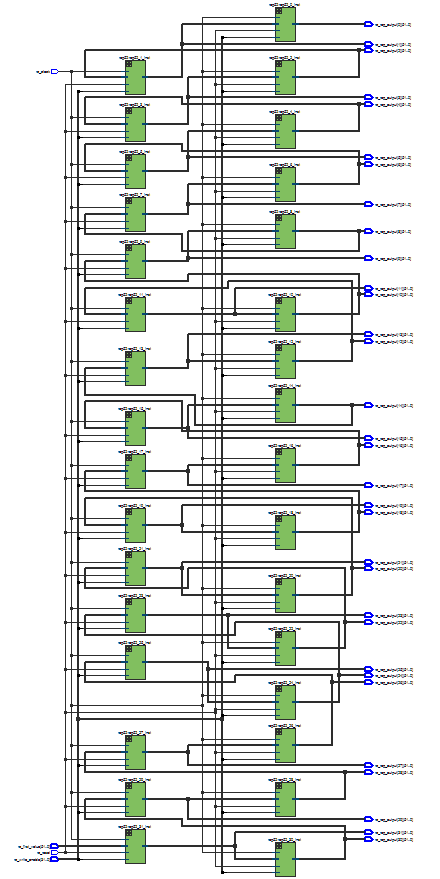
\includegraphics[width=0.5\textwidth]{register_chain_rtl.PNG}
  \caption{RTL of Register Chain}
  \label{fig:regchain-rtl}
\end{figure}

\newpage
\subsubsection{Compare Module}

The compare module is used to match address with the contents of the register chain. The address matched could either be the source address or the destination address. The module implementation can be found in \texttt{compare.vhd}. Table~\ref{tab:compare} shows the signal names of the intra-subsystem interface. 


\begin{table}[ht]
    \begin{center}
        \begin{tabular}{lll}\hline
        Signal & Type & In/Out \\
        \hline
        \texttt{cmp\_address\_to\_compare} & std\_logic\_vector(47 downto 0) & In \\
        \hline
        \texttt{cmp\_reg\_output\_address} & reg\_output\_type & In \\
        \hline
        \texttt{cmp\_compare\_result} & std\_logic\_vector(31 downto 0) & Out \\
        \hline
        \end{tabular}
        \caption{Compare Interface}\label{tab:compare}
    \end{center}
\end{table}

The \texttt{cmp\_address\_to\_compare} signal is a 48-bit vector which contains the address which we are comparing the register chain addresses to. 

The \texttt{cmp\_reg\_output\_address} is of type \texttt{reg\_output\_type} which is a 32 by 52 bit two-dimensional vector that is the output of the register chain module. The 48 MAC address bits of each 52 bit vector is being compared to the \texttt{cmp\_address\_to\_compare} signal. 

The \texttt{cmp\_compare\_result} is a 32 bit output which asserts which register files' addresses match the \texttt{cmp\_address\_to\_compare}. By design of the register chain, there can only be one match or zero matches. The 31st bit of the output represents the comparison result of the left-most register file and the 1st bit of the output represents the comparison result of the right-most register file.

The RTL of the compare module is shown in Figure~\ref{fig:compare-rtl}. The RTL shows 32 48-bit comparators in parallel.

\begin{figure}[ht!]
  \centering
  	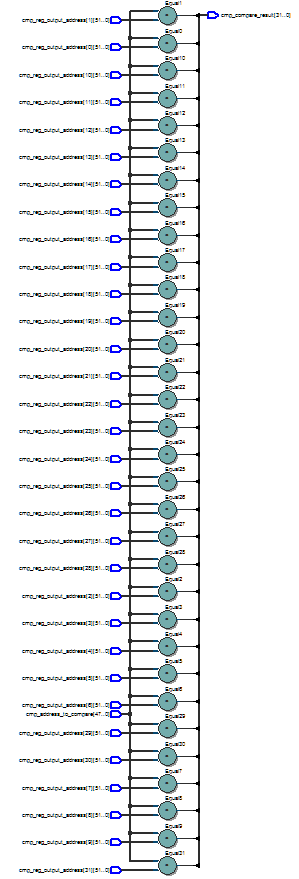
\includegraphics[width=0.25\textwidth]{compare_rtl.PNG}
  \caption{RTL of Compare Module}
  \label{fig:compare-rtl}
\end{figure}

\newpage
\subsubsection{Compute Module}

The compute module is used to determine the 52-bit \texttt{first\_value} and 32-bit \texttt{write\_enable} input signals for the register chain. To perform this calculation, it uses the current state of the FSM (described in section \ref{fsm}), the 32 by 52 bit two-dimensional output of the register chain, and the 32-bit comparison result calculated by the compare module. The module implementation can be found in \texttt{compute.vhd}. Table~\ref{tab:compute} shows the signal names of the intra-subsystem interface. 

\begin{table}[ht]
    \begin{center}
        \begin{tabular}{lll}\hline
        Signal & Type & In/Out \\
        \hline
        \texttt{cpt\_state} & state\_type & In \\
        \hline
        \texttt{cpt\_reg\_output\_address} & reg\_output\_type & In \\
        \hline
        \texttt{cpt\_compare\_result} & std\_logic\_vector(31 downto 0) & In \\
        \hline
        \texttt{cpt\_first\_value} & std\_logic\_vector(51 downto 0) & Out \\
        \hline
        \texttt{cpt\_write\_enable} & std\_logic\_vector(31 downto 0) & Out \\
        \hline
        \end{tabular}
        \caption{Compute Interface}\label{tab:compute}
    \end{center}
\end{table}

The \texttt{cpt\_state} signal represents the current state of the FSM as defined in section \ref{fsm}. The possible states are \texttt{reset\_state}, \texttt{read\_state}, and \texttt{write\_state}. The compute module outputs different signals depending on whether we are in the reset (idle), load (reset), or store (write) states.

The \texttt{cpt\_reg\_output\_address} signal is simply the output of the register chain as previously defined.

The \texttt{cpt\_first\_value} signal is a 52-bit vector that is the input to the register chain. It represents the value that should be written into the left-most register file. This value only holds significance in the read state (load) as the write state (store) simply uses the new address and port. This value is the address stored at the register file where the match was found. Generating this signal was the most technically challenging aspect of the entire project. Three different designs were implemented and one was selected in the end.

\begin{enumerate}
\item
The selected design (third and final design) took advantage of a large amount of parallel hardware. First, a 32 by 52 bit two-dimensional vector (same size as register chain output) was generated. Each of the 52-bit vectors in this temporary signal was set to all 1s if the $i$th \texttt{cpt\_compare\_result} value was asserted. If the $i$th value was not asserted, the temporary signal at that index was simply all 0s. Then, for each of the 52 indices in the 52-bit vectors, all 32 bits at the index (0 to 51) were OR'd together to generate a 52-bit \texttt{cpt\_first\_value} output. 
\item
Another design (second design) converted the 32-bit \texttt{cpt\_compare\_result} from its one-hot encoding (only up to one match can be found) into a natural number. This conversion was performed using an \texttt{if-else} chain where each bit from 31 to 0 was compared to 1 and the corresponding natural number was returned. In the case where there was no match (address not found), the number 31 was returned, but this value has no significance as the value is not used when no match is found (we don't do anything to the register chain when we don't find an address in load and we store the new address and port in a store operation). The natural number was then used to select a 52-bit vector by index using VHDL language constructs. 
\item
The original design was similar to the second described design except that the \texttt{cpt\_first\_value} was directly assigned in each body of the \texttt{if-else} chain, resulting in significantly increased logic gate usage. 
\end{enumerate}

In the end, the three designs were compared using compilation time and logic gate usage as metrics. The second design used the fewest logic gates, but had a significantly (2 times) longer compilation time, so the first design was used. The third (original) design was worse by every metric. 

The \texttt{cpt\_write\_enable} signal is a 32-bit vector that leads to the register chain write-enable signal. This signal is state-dependent. In the reset state, the signal is simply all 0s. In the read state, we assert all the bits left of the asserted bit in the \texttt{cpt\_compare\_result} vector, inclusive. This way, we overwrite all the register files left of and including the register file where we found the address matching the destination address. Note that the implementation still works when none of the \texttt{cpt\_compare\_result} vector bits are asserted since then none of the \texttt{cpt\_write\_enable} bits will be asserted, which is the expected behavior. In the write state, asserting all the bits left of the asserted bit in the \texttt{cpt\_compare\_result} vector still works when we do find a match. The write state differs from the read state when we do not find the address. In the write state, when we do not find the address, we simply assert every bit in the \texttt{cpt\_write\_enable} vector since all register chain contents will be shifted to make room for the new address and the least recently used address to port mapping will be evicted.

The RTL of the compute module is shown in Figure~\ref{fig:compute-rtl}. The RTL shows the parallel muxes for the first stage of the \texttt{first\_value} signal processing and OR gates for the second stage. For the \texttt{write\_enable} signal, the left-hot encoder is RTL'd into a series of comparators whose outputs feed into muxes. 

\begin{figure}[ht!]
  \centering
  	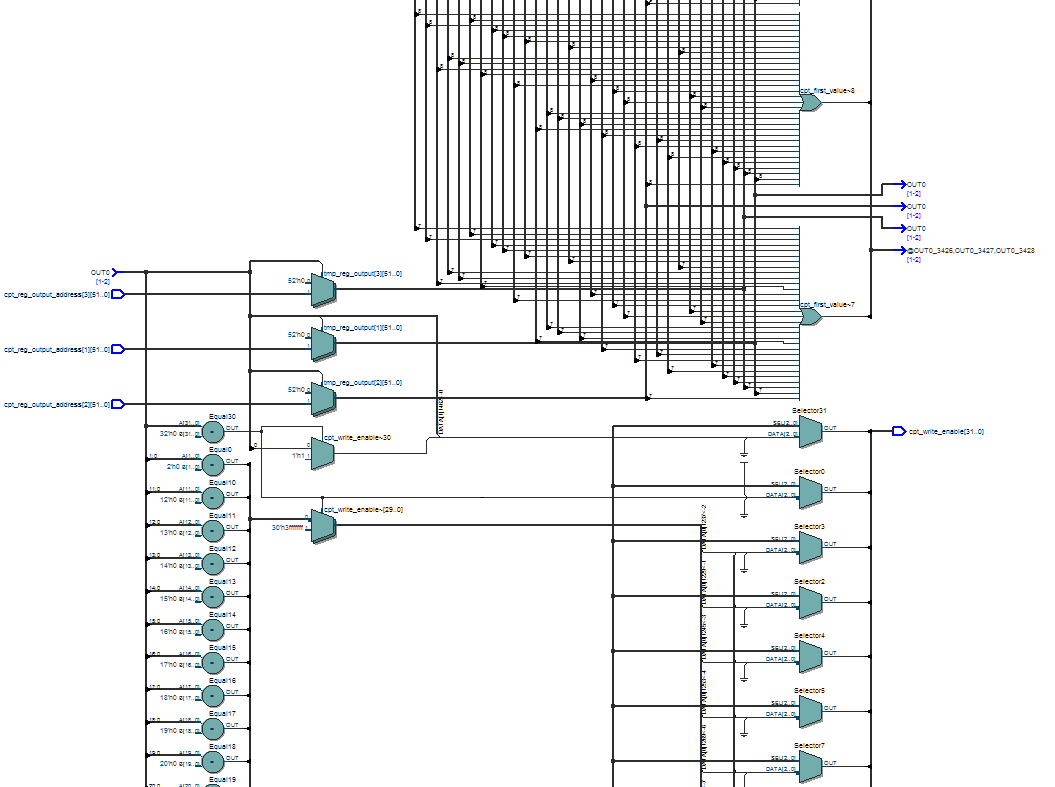
\includegraphics[width=0.75\textwidth]{compute_rtl.PNG}
  \caption{RTL of Compute Module}
  \label{fig:compute-rtl}
\end{figure}

\newpage
\subsubsection{FSM Module} \label{fsm}

The \texttt{FSM} module is responsible for outputting control signals and latching outputs to be output at the correct times. The state output of the FSM is used in other modules to determine which datapaths to use. The three possible states are reset (table is idle and awaiting trigger), read (table is trying to find the destination address and return a port), and write (table is storing the new source address and port). The module implementation can be found in \texttt{fsm.vhd}. Table~\ref{tab:fsm} shows the signal names of the intra-subsystem interface. 

\begin{table}[ht]
    \begin{center}
        \begin{tabular}{lll}\hline
        Signal & Type & In/Out \\
        \hline
        \texttt{fsm\_clock} & std\_logic & In \\
        \hline
        \texttt{fsm\_reset} & std\_logic & In \\
        \hline
        \texttt{fsm\_trigger} & std\_logic & In \\
        \hline
        \texttt{fsm\_compute\_output} & std\_logic\_vector(3 downto 0) & In \\
        \hline
        \texttt{fsm\_not\_found} & std\_logic & In \\
        \hline
        \texttt{fsm\_state} & state\_type & Out \\
        \hline
        \texttt{fsm\_input\_ready} & std\_logic & Out \\
        \hline
        \texttt{fsm\_output\_ready} & std\_logic & Out \\
        \hline
        \texttt{fsm\_destination\_port} & std\_logic\_vector(3 downto 0) & Out \\
        \hline
        \end{tabular}
        \caption{FSM Interface}\label{tab:fsm}
    \end{center}
\end{table}

The \texttt{fsm\_clock} and \texttt{fsm\_reset} signals are passed to the FSM module from the inter-subsystem interface. The positive clock edge is used to advance state (by assigning next state to current state) while the asynchronous reset signal is used to put the FSM back in the reset state. 

The \texttt{fsm\_trigger} signal is also passed directly from the inter-subsystem interface and is used to determine the next state. When the FSM is in the reset state, if the \texttt{fsm\_trigger} signal is asserted, then the next state is the read state. If the \texttt{fsm\_trigger} signal is not asserted, then the next state is simply the reset state. These state transitions are covered in detail in Figure~\ref{fig:fsm-transition}. The state transition diagram shows how the \texttt{trigger} input affects the next-state. Note that the next-state becomes the current state only upon the positive clock edge, so the only point in time the \texttt{trigger} is relevant is during the positive clock edge.

\begin{figure}[ht!]
  \centering
  	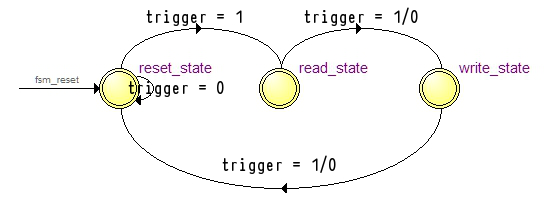
\includegraphics[width=0.75\textwidth]{fsm_updated_state_transition_diagram.PNG}
  \caption{FSM State Transition Diagram}
  \label{fig:fsm-transition}
\end{figure}

For clarity, Table~\ref{tab:fsm-table} shows the transition cases in tabular form.

\begin{table}[ht]
    \begin{center}
        \begin{tabular}{lll}\hline
        Source State & Destination State & Condition \\
        \hline
        reset & reset & trigger = 0 and positive clock edge \\
        \hline
        reset & read & trigger = 1 and positive clock edge \\
        \hline
        read & write & positive clock edge \\
        \hline
        write & reset & positive clock edge \\
        \hline
        \end{tabular}
        \caption{FSM Transition Table}\label{tab:fsm-table}
    \end{center}
\end{table}

The \texttt{fsm\_compute\_output} signal is the 4-bit vector representing the port found (as part of the 52 bit register file contents) during the read state within the compute module. It is used to generate and correctly latch the \texttt{fsm\_destination\_port} output signal.

The \texttt{fsm\_not\_found} signal is calculated in the address table wrapper and is asserted when the compare module output is all 0s, showing that the destination address was not found. The \texttt{fsm\_not\_found} signal is used to set the destination port to "1111" when the destination address is not found.

The \texttt{fsm\_state} signal is an output representing the current state. The state is used within the wrapper module as well as in the compute module.

The \texttt{fsm\_input\_ready} signal is an output control signal asserting that the table is ready to process a new load-store operation. The signal is asserted when the FSM is in the reset state and de-asserted in the read and write states.

The \texttt{fsm\_output\_ready} signal is an output control signal asserting that the table has generated a destination port. The signal is asserted when the FSM is in the write state. This seems incorrect, but the inter-subsystem interface defines the destination port being valid at the positive edge of the \texttt{output\_ready} signal and the destination port will not change during the read state to write state transition, so the port will be valid at this edge.

The \texttt{fsm\_destination\_port} signal is the output signal that is exposed in the inter-subsystem interface. It is presented as a 4-bit one-hot encoded port if the destination address was successfully found and as "1111" if not found. Note that since this signal must be valid at the positive edge of the \texttt{output\_ready} signal which is directly triggered by the positive clock edge, we change the \texttt{destination\_port} signal on the negative clock edge so there are no race conditions. The value the signal takes on when we do find a destination address is simply the 4 port bits of the 52-bit register file contents that yielded a successful comparison with the destination address.

The RTL of the FSM is shown in Figure~\ref{fig:fsm-rtl}. The RTL is fairly self-explanatory and most importantly contains the state register which stores the current state of the FSM.

\begin{figure}[ht!]
  \centering
  	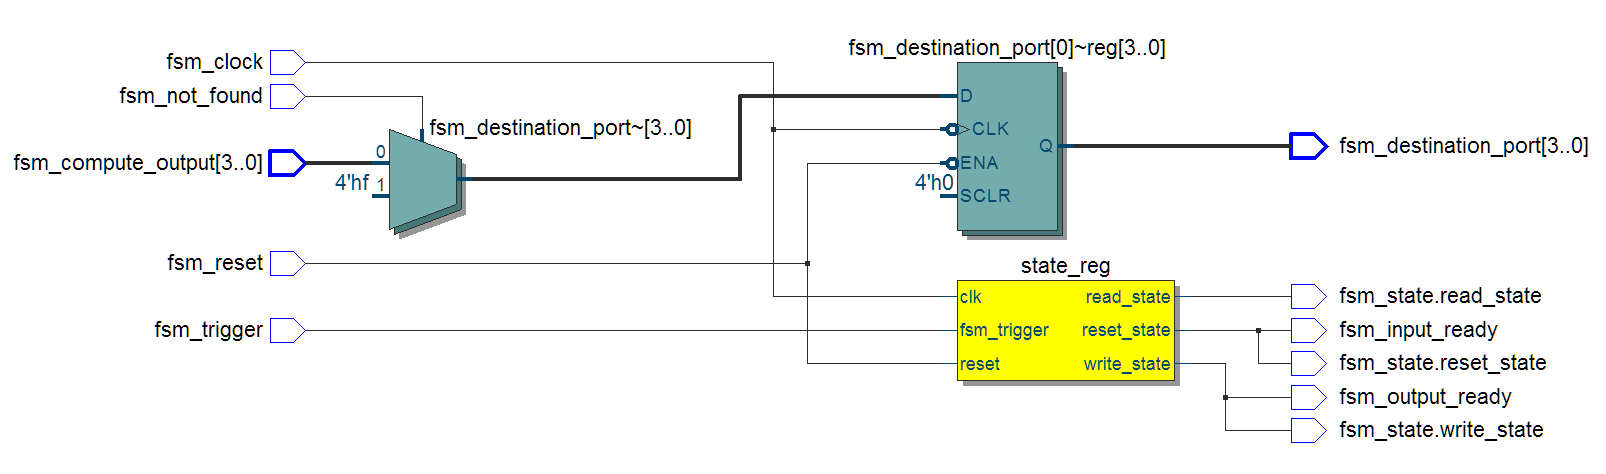
\includegraphics[width=1.0\textwidth]{fsm_rtl.PNG}
  \caption{RTL of FSM}
  \label{fig:fsm-rtl}
\end{figure}

\subsubsection{Address Table Module}

The address table module is simply a wrapper that contains the inter-subsystem interface definitions in addition to the mappings and instantiations of all the intra-subsystem modules. The wrapper also takes care of certain functionalities that don't belong in any other modules, such as latching inputs and error correcting. The wrapper implementation can be found in \texttt{address\_table.vhd}.

The main use of the wrapper module is to connect all the intra-subsystem modules together. The four modules instantiated in the wrapper are FSM, register-chain, compare, and compute. 

The wrapper latches inputs in two layers. This is because we must keep the latched inputs (source address, source port, destination address) active for two clock cycles since the values must be valid for both the read state (first cycle) and write state (second cycle). This is performed using two sequentially chained latches with the output of the first latch used for the read state and the output of the second layer used for the write state.

The wrapper is also used to perform some minor error correction. This "error correction" is more "error prevention" than strict error correction. One place this error prevention is used is during the assertion of asynchronous reset. When the \texttt{reset} signal is asserted, all other inputs are simply ignored and set to all 0s. Additionally, depending on state, certain module input signals and inter-subsystem interface signals are hardcoded, such as setting \texttt{write\_enable} to all 0s in the reset state and setting \texttt{monitor\_access} to 1 during only the read state. These signals should already have their hardcoded values, but this check simply ignores any potentially incorrect values, saving time in development. In a more strict production environment, these error prevention snippets would be removed and the output signals for the subsystems would be more vigorously tested.

The RTL for the entire subsystem is shown in Figure~\ref{fig:table-rtl}. The RTL shows all the internal modules in addition to the processes that occur in the wrapper itself.

\begin{figure}[ht!]
  \centering
  	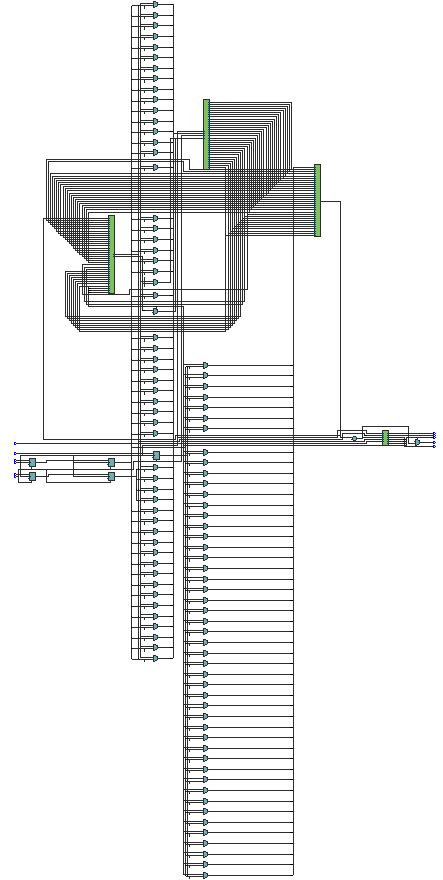
\includegraphics[width=0.5\textwidth]{table_rtl.PNG}
  \caption{RTL of Table Subsystem}
  \label{fig:table-rtl}
\end{figure}

\newpage
\section{Simulation Results}

Timing simulations were run on the full subsystem. Every input and output signal defined in the inter-subsystem interface was monitored. The basic simulation (Figures 7 and 8) tested the following functionalities:

\begin{enumerate}
\item A stored address-port mapping can be retrieved a trigger-cycle after it is stored.
\item A stored address-port mapping can be retrieved multiple trigger-cycles after it is stored.
\item A stored address-port mapping can be replaced with a new port
\item The destination port is valid upon the positive edge of the \texttt{output\_ready} signal
\item The destination port shows "1111" when the address does not exist in the table
\item \texttt{input\_ready} is asserted at the correct time
\item \texttt{monitor\_access} and \texttt{monitor\_not\_found} are asserted during a positive clock edge
\end{enumerate}

\begin{figure}[ht!]
  \centering
  	\includegraphics[width=0.95\textwidth]{complete_test1.png}
  \caption{First complete test demonstrating functionalities 1, 2, and 5}
  \label{fig:complete-test1}
\end{figure}

\begin{figure}[ht!]
  \centering
  	\includegraphics[width=0.95\textwidth]{complete_test2.png}
  \caption{Second complete test demonstrating functionalities 3, 4, 6, and 7}
  \label{fig:complete-test2}
\end{figure}

\newpage

A longer waveform simulation (Figure 9) was also performed and tested that addresses that are not read or written to (updated) are evicted from the table.

\begin{figure}[ht!]
  \centering
  	\includegraphics[width=0.95\textwidth]{eviction_test.png}
  \caption{Demonstration of address eviction}
  \label{fig:eviction-test}
\end{figure}

In addition to simulating the full subsystem, the following tests were also run on individual modules to confirm their correct operation:
\begin{enumerate}
\item The compare module correctly selects the register with a matching source address. This test demonstrates that we will correctly select the register whose address matches the one inputted by forwarding.

\begin{figure}[ht!]
  \centering
  	\includegraphics[width=0.95\textwidth]{compare.png}
  \caption{Test of the compare module}
  \label{fig:eviction}
\end{figure}

\item The compute module correctly shifts the correct number of registers while it is in the read state and a matching register has been found. This test demonstrates that we will correctly write-enable the proper registers in our register-chain.

\begin{figure}[ht!]
  \centering
  	\includegraphics[width=0.95\textwidth]{compute_read.png}
  \caption{Test of the compute module in the read state}
  \label{fig:compute_read}
\end{figure}

\newpage

\item The compute module shifts all of the registers when it is in the write state and a matching register has not been found. Important for ensuring that old values will eventually become evicted from the register chain since the resulting signal will write-enable every register in the chain.

\begin{figure}[ht!]
  \centering
  	\includegraphics[width=0.95\textwidth]{compute_write.png}
  \caption{Test of the compute module in the write state}
  \label{fig:compute_write}
\end{figure}

\item The register chain will propagate a value entered into its first register, critical for the fundamental operation of the eviction system.

\begin{figure}[ht!]
  \centering
  	\includegraphics[width=0.95\textwidth]{rc_propagate.png}
  \caption{Test of address propagation in the register chain}
  \label{fig:rc_propagate}
\end{figure}

\end{enumerate}

\section{Hardware Test Results}

Two separate testing utilities were implemented. The first was simply an interface with the DE0-CV FPGA inputs and outputs allowing the table functionality to be tested by a human. The second was a more sophisticated memory-based test that read inputs and expected outputs from a ROM with user-defined programatically generated values.

\subsubsection{Human Interface Test}

The human interface test was implemented to test the functionality of the table in hardware. The inter-subsystem interface inputs and outputs were all connected to signals in a test wrapper, which abstracted all the signals into hardware inputs and outputs. Table~\ref{tab:test1} shows the signal names of the hardware interface. The implementation of this test can be found in \texttt{address\_table\_hardware\_test}.  

\begin{table}[ht]
    \begin{center}
        \begin{tabular}{lll}\hline
        Signal & Type & In/Out \\
        \hline
        \texttt{test\_clock} & std\_logic & In \\
        \hline
        \texttt{test\_reset} & std\_logic & In \\
        \hline
        \texttt{test\_source\_address} & std\_logic\_vector(2 downto 0) & In \\
        \hline
        \texttt{test\_source\_port} & std\_logic\_vector(3 downto 0) & In \\
        \hline
        \texttt{test\_destination\_address} & std\_logic\_vector(2 downto 0) & In \\
        \hline
        \texttt{test\_push\_pin} & std\_logic & In \\
        \hline
        \texttt{test\_destination\_port} & std\_logic\_vector(3 downto 0) & Out \\
        \hline
        \texttt{test\_not\_found} & std\_logic & Out \\
        \hline
        \end{tabular}
        \caption{Human-interface Test Interface}\label{tab:test1}
    \end{center}
\end{table}

The \texttt{text\_clock} signal can either be wired to a push-pin to manually clock the table or to the 50 MHz FPGA clock. Using the 50 MHz FPGA clock means losing out on the transitions between the reset, read, and write states, but still behaves just like in the static way, with the final resting state shown. 

The \texttt{test\_reset} signal is wired to a push-pin and is used to reset the contents of the table.

The \texttt{test\_source\_address}, \texttt{test\_source\_port}, and \texttt{test\_destination\_address} signals are wired to switches. The addresses are 3 bits wide each and the port is 4 bits wide to allow us to fully utilize the 10 available switches. The 3 bits simply represent the three least significant bits of the 48-bit MAC address.

The \texttt{test\_push\_pin} signal is wired to a push-pin. This signal, which can be asserted for many cycles (for as long as a user holds it down), is "debounced" into a single negative edge clocked \texttt{trigger} signal which is used by the table. The debouncing is performed by an FSM which can be examined in detail by looking at the source file.

The \texttt{test\_destination\_port} signal is the destination port output of the table and is latched at the positive edge of the \texttt{output\_ready} signal. This signal persists until the next latching of the signal. The output is displayed on four LEDs.

The \texttt{test\_not\_found} signal is asserted when the all four bits of the \texttt{test\_destination\_port} signal are asserted, signifying that a destination address was not found.

\subsubsection{Memory-based Test}

While the human-interface test was sufficient for demonstrating that the table worked by manually setting inputs and validating outputs, it is not a reliable way of verifying operations such as eviction due to the huge number of operations and potential for human error. Because of this, a memory-based hardware test was designed and implemented to allow tests to be written using ROM.

The memory-based test has a ROM module that contains 1024 rows of 128-bit data. Each row contains data in the format defined in Table~\ref{tab:rom}. 

\begin{table}[ht]
    \begin{center}
        \begin{tabular}{lll}\hline
        Bits & Input/Expected Output & Description \\
        \hline
        [47:0] & Input & \texttt{source\_address} \\
        \hline
        [95:48] & Input & \texttt{destination\_address} \\
        \hline
        [99:96] & Input & \texttt{source\_port} \\
        \hline
        [103:100] & Expected Output & \texttt{destination\_port} \\
        \hline
        [104] & Expected Output & \texttt{monitor\_access} \\
       	\hline
        [105] & Expected Output & \texttt{monitor\_not\_found} \\
        \hline
        [127:106] & N/A & Empty (all 0s) \\
        \hline
        \end{tabular}
        \caption{ROM Format}\label{tab:rom}
    \end{center}
\end{table}

The memory-based test has a hardware interface defined in Table~\ref{tab:test2}

\begin{table}[ht]
    \begin{center}
        \begin{tabular}{lll}\hline
        Signal & Type & In/Out \\
        \hline
        \texttt{hwtest\_clock} & std\_logic & In \\
        \hline
        \texttt{hwtest\_reset} & std\_logic & In \\
        \hline
        \texttt{hwtest\_access\_count} & std\_logic\_vector(7 downto 0) & Out \\
        \hline
        \texttt{hwtest\_not\_found\_count} & std\_logic\_vector(7 downto 0) & Out \\
        \hline
        \texttt{hwtest\_access\_incorrect} & std\_logic\_vector(7 downto 0) & Out \\
        \hline
        \texttt{hwtest\_not\_found\_incorrect} & std\_logic\_vector(7 downto 0) & Out \\
        \hline
        \texttt{hwtest\_destination\_port\_incorrect} & std\_logic\_vector(7 downto 0) & Out \\
        \hline
        \end{tabular}
        \caption{Memory-based Test Format}\label{tab:test2}
    \end{center}
\end{table}

The \texttt{hwtest\_clock} signal can either be connected to the 50 MHz clock or a manual push-pin clock. The \texttt{hwtest\_reset} signal should be wired to a push-pin.

The \texttt{hwtest\_access\_count} signal is an 8-bit value (0-255) representing the number of times the table was accessed.

The \texttt{hwtest\_not\_found\_count} signal is an 8-bit value representing the number of times the destination port was not found.

The \texttt{hwtest\_access\_incorrect} signal is an 8-bit value representing the number of times the access signal from the table differed from expected.

The \texttt{hwtest\_not\_found\_incorrect} signal is an 8-bit value representing the number of times the not-found signal from the table differed from expected.

The \texttt{hwtest\_destination\_port\_incorrect} signal is an 8-bit value representing the number of times the \texttt{destination\_port} signal differed from expected.

The memory-based test runs off a cycle-counter, which is a sequential circular FSM and an address-counter. The cycle-counter starts at 0 and increments once every clock cycle, but only the 3 least significant bits of the cycle-counter are considered. The ROM element takes the address-counter and clock as inputs and outputs a 128-bit vector which is dissected into all the inputs and expected outputs. The table \texttt{trigger} input is asserted at the negative clock edge in the second state of the cycle-counter. The signal is then de-asserted at the negative clock edge in the third state of the cycle-counter. At the negative edge of the seventh state of the cycle-counter, the address-counter is incremented so we can run the next load-store operation. 

Since the \texttt{destination\_port} output of the table is only valid at the positive edge of the \texttt{output\_ready} output, the output at that point is compared to the expected destination port. If the value is different from expected, the \texttt{hwtest\_destination\_port\_incorrect} counter is incremented by one.

The \texttt{hwtest\_access\_count} and \texttt{hwtest\_not\_found\_count} counters are incremented every time the \texttt{monitor\_access} and \texttt{monitor\_not\_found} signals, respectively, are asserted on the positive clock edge. 

Since the \texttt{monitor\_access} and \texttt{monitor\_not\_found} signals can be asserted at any clock cycle between when the \texttt{trigger} signal is clocked and the \texttt{output\_ready} signal is asserted, we use a register to hold each of these values and latch an assertion if one occurs. These two registers are cleared on the positive clock edge in the first state of the cycle-counter. The registers are compared to the expected \texttt{access} and \texttt{not\_found} values on the negative clock edge of the sixth state of the cycle-counter.

There exist a few more nuances that can be seen in the \texttt{address\_table\_hardware\_memory\_test.vhd} file. Figure~\ref{fig:hardware_1} shows correct operation of the table. Note that the incorrect counters remain at 0 even as \texttt{access} and \texttt{not\_found} counters increase.

\begin{figure}[ht!]
  \centering
  	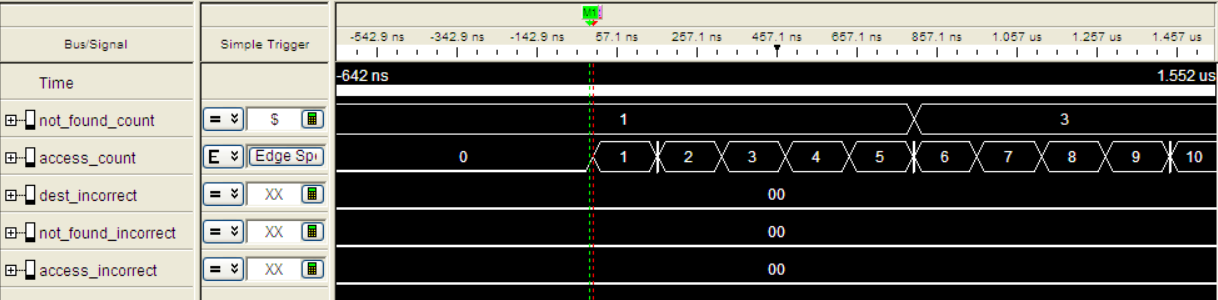
\includegraphics[width=0.95\textwidth]{hardware_1.PNG}
  \caption{Logic Analyzer Output Showing Correct Table Operation}
  \label{fig:hardware_1}
\end{figure}

Figure~\ref{fig:hardware_2} shows correct operation of the eviction functionality of the table. Note that the \texttt{not\_found} counter increases while the incorrect counters remain at 0. The test case can be found in the \texttt{MIF} file and the Go script.

\begin{figure}[ht!]
  \centering
  	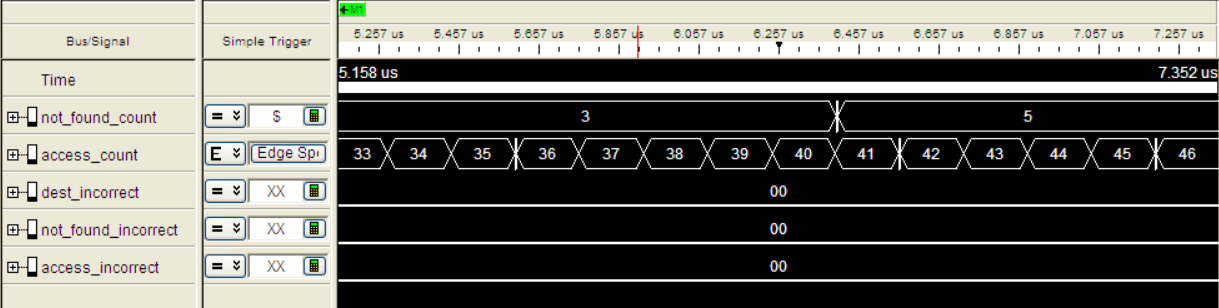
\includegraphics[width=0.95\textwidth]{hardware_2.PNG}
  \caption{Logic Analyzer Output Showing Correct Table Eviction Operation}
  \label{fig:hardware_2}
\end{figure}

\section{Conclusion}

We were able to verify the functionality of our table subsystem through both software and hardware tests. Interfacing with the forwarding subsystem was completely seamless and the table functioned correctly as part of the forwarding system. Overall, we enjoyed creating a core subsystem of an ethernet switch.

\end{document}
